\documentclass[10pt]{beamer}

%%%
% PREAMBLE FOR THIS DOC 
%%%
%https://tex.stackexchange.com/questions/68821/is-it-possible-to-create-a-latex-preamble-header
\usepackage{/Users/miw267/Repos/latex_preamble/beamer_preamble}

\usetikzlibrary{matrix}



% \album{image file}{url}{artist}{album}
\newcommand{\album}[4]{%
  \begin{minipage}[t]{0.185\textwidth}\centering
    \href{#2}{\includegraphics[width=\linewidth]{#1}}\\[0.3em]
    {\small\bfseries #3}\\{\small #4}
  \end{minipage}}
  
\newcommand{\albumtiny}[4]{%
  \begin{minipage}[t]{0.185\textwidth}\centering
    \href{#2}{\includegraphics[width=\linewidth]{#1}}\\[0.3em]
    {\tiny \bfseries #3}\\{\tiny #4}
  \end{minipage}}
  
  
%%%
% DOCUMENT
%%%

\begin{document}

%\maketitle

%% Title page frame
%\begin{frame}
%    \titlepage 
%\end{frame}





\title{09/30/2026: Binomial Coefficients}
\author{CSCI 246: Discrete Structures}
\date{Textbook reference: Sec 17, Scheinerman}

\begin{frame}
    \titlepage 
\end{frame}


\begin{frame}

%\begin{myredbox}[title=Announcements]
%\begin{itemize}
%	\item The guest instructor for today is Associate Professor Sean Yaw. Mike W. is giving a research talk from 4-5pm at the MSU Technology and Artificial Intelligence Learning Seminar (TAILS). 
%\end{itemize}
%\end{myredbox}
%\vfill 


\begin{myyellowbox}[title=Today's Agenda]
\begin{itemize}
	\item Mini-lecture (30 mins)
	\item Group exercises (20 mins)
%	%
%	\begin{itemize}
%	\footnotesize 
%	\item Review induction 
%	\end{itemize}
%	%
\end{itemize}

%	Rationale for group exercises: we got shortchanged on time last couple days, and I already did a lot of lectures, so I want you to practice. Next problems quiz will cover relations and functions: Hamkins and 
%	
\end{myyellowbox}
\vfill 

\end{frame}


\begin{frame}{Study Guide For Quiz 5}
\footnotesize 

\colorbox{yellow!20}{\textbf{Group exercises.}} Know how to do all of the group exercises from the course meetings on Relations (9/23), Equivalence Relations (9/25), and Partitions (9/28).


\vfill 

\colorbox{red!20}{\textbf{Readings.}} 
Sec. 14 (Relations)
\begin{itemize}
\item Understand the definition of relations in Def 14.2.
\item Know how to determine whether a relation is reflexive, symmetric, and/or transitive, as in Examples 14.8-14.11.  (Skip antisymmetric and irreflexive.)
\end{itemize}
Sec. 15 (Equivalence Relations)
\begin{itemize}
\item Know how to apply the definition of congruence mod $n$ (to determine whether a pair of numbers is congruent).
\item Know how to prove that congruence mod $n$ is an equivalence relation.
\item Know how to determine equivalence classes as in Examples 15.7 and 15.8.
\end{itemize}
Sec. 16 (Partitions)
\begin{itemize}
\item Understand how partitions and equivalence classes are \qq{two sides of the same coin}.
\item Know how to count the number of ways to rearrange the letters in the words \texttt{WORD}, \texttt{HELLO}, and \texttt{AARDVARK}, and justify your answer using equivalence classes.
\end{itemize}

\end{frame}


\begin{frame}[standout]
Binomial Coefficients	
\end{frame}


\begin{frame}{Five albums}
\only<1>{\colorbox{yellow!30}{\textbf{Activity.}} As we listen to clips from these five albums, think about how would you sort them in terms of how much you like them.
\vfill 
}


\only<1>{
\begin{center}
\album{images/gkmc}{https://open.spotify.com/track/1jpEnbAJkcI30exvaUM60R?si=2c0c0227a6524fb4}{Kendrick Lamar}{good kid, m.A.A.d city}\hfill
\album{images/folklore}{https://open.spotify.com/track/6nK2pIKFcRc5frrZKHgsiT?si=9a04921ac10b41c2}{Taylor Swift}{folklore}\hfill
\album{images/invisible_cinema}{https://open.spotify.com/track/3pHi49H2DjfnpqX6iOaLC8?si=2bc151d028694816}{Aaron Parks}{Invisible Cinema}\hfill
\album{images/midwest_princess}{https://open.spotify.com/track/0PCQjOXi4yORRcXHrOAxaK?si=145894a1b6fa4d3b}{Chappell Roan}{The Rise and Fall of a Midwest Princess}\hfill
\album{images/zach_bryan}{https://open.spotify.com/track/00syWkRGIVQvYsg2OwfBUw?si=4fcfc29614034924}{Zach Bryan}{Zach Bryan}
\end{center}
}

\only<2->{
\begin{center}
\albumtiny{images/gkmc}{https://open.spotify.com/track/1jpEnbAJkcI30exvaUM60R?si=2c0c0227a6524fb4}{Kendrick Lamar}{good kid, m.A.A.d city}\hfill
\albumtiny{images/folklore}{https://open.spotify.com/track/6nK2pIKFcRc5frrZKHgsiT?si=9a04921ac10b41c2}{Taylor Swift}{folklore}\hfill
\albumtiny{images/invisible_cinema}{https://open.spotify.com/track/3pHi49H2DjfnpqX6iOaLC8?si=2bc151d028694816}{Aaron Parks}{Invisible Cinema}\hfill
\albumtiny{images/midwest_princess}{https://open.spotify.com/track/0PCQjOXi4yORRcXHrOAxaK?si=145894a1b6fa4d3b}{Chappell Roan}{The Rise and Fall of a Midwest Princess}\hfill
\albumtiny{images/zach_bryan}{https://open.spotify.com/track/00syWkRGIVQvYsg2OwfBUw?si=4fcfc29614034924}{Zach Bryan}{Zach Bryan}
\end{center}
\vfill 
}


\only<2->{
\colorbox{yellow!30}{\textbf{Activity.}} Find a partner and answer these questions: 
\begin{enumerate}
	\item How many ways are these to rank (sort) these five albums?
	\item How many ways are there to pick a favorite and second favorite album?
	\item How many ways are there to pick 2 (different) albums for a road trip to Helena?
\end{enumerate}
}
\end{frame}


\begin{frame}{Number of ways to rank the five albums}

\footnotesize The number of ways to sort (rank) all five albums is
\[ 5 \cdot 4 \cdot 3 \cdot 2 \cdot 1. \]

To see this, let's use the shorthand:
\textbf{K}endrick \quad \textbf{T}aylor \quad \textbf{A}aron \quad \textbf{C}happell \quad \textbf{Z}ach

\begin{center}

\tiny\ttfamily
\setlength{\tabcolsep}{16pt}\renewcommand{\arraystretch}{0.95}
\begin{tabular}{ccccc}
\textbf{\color{blue!70!black}K\,\ldots} & \textbf{\color{orange!80!black}T\,\ldots} & \textbf{\color{green!45!black}A\,\ldots} & \textbf{\color{red!70!black}C\,\ldots} & \textbf{\color{purple!70!black}Z\,\ldots} \\[1pt]
\hline
{\color{blue!70!black}KTACZ} & {\color{orange!80!black}TKACZ} & {\color{green!45!black}AKTCZ} & {\color{red!70!black}CKTAZ} & {\color{purple!70!black}ZKTAC} \\
{\color{blue!70!black}KTAZC} & {\color{orange!80!black}TKAZC} & {\color{green!45!black}AKTZC} & {\color{red!70!black}CKTZA} & {\color{purple!70!black}ZKTCA} \\
{\color{blue!70!black}KTCAZ} & {\color{orange!80!black}TKCAZ} & {\color{green!45!black}AKCTZ} & {\color{red!70!black}CKATZ} & {\color{purple!70!black}ZKATC} \\
{\color{blue!70!black}KTCZA} & {\color{orange!80!black}TKCZA} & {\color{green!45!black}AKCZT} & {\color{red!70!black}CKAZT} & {\color{purple!70!black}ZKACT} \\
{\color{blue!70!black}KTZAC} & {\color{orange!80!black}TKZAC} & {\color{green!45!black}AKZTC} & {\color{red!70!black}CKZTA} & {\color{purple!70!black}ZKCTA} \\
{\color{blue!70!black}KTZCA} & {\color{orange!80!black}TKZCA} & {\color{green!45!black}AKZCT} & {\color{red!70!black}CKZAT} & {\color{purple!70!black}ZKCAT} \\
{\color{blue!70!black}KATCZ} & {\color{orange!80!black}TAKCZ} & {\color{green!45!black}ATKCZ} & {\color{red!70!black}CTKAZ} & {\color{purple!70!black}ZTKAC} \\
{\color{blue!70!black}KATZC} & {\color{orange!80!black}TAKZC} & {\color{green!45!black}ATKZC} & {\color{red!70!black}CTKZA} & {\color{purple!70!black}ZTKCA} \\
{\color{blue!70!black}KACTZ} & {\color{orange!80!black}TACKZ} & {\color{green!45!black}ATCKZ} & {\color{red!70!black}CTAKZ} & {\color{purple!70!black}ZTAKC} \\
{\color{blue!70!black}KACZT} & {\color{orange!80!black}TACZK} & {\color{green!45!black}ATCZK} & {\color{red!70!black}CTAZK} & {\color{purple!70!black}ZTACK} \\
{\color{blue!70!black}KAZTC} & {\color{orange!80!black}TAZKC} & {\color{green!45!black}ATZKC} & {\color{red!70!black}CTZKA} & {\color{purple!70!black}ZTCKA} \\
{\color{blue!70!black}KAZCT} & {\color{orange!80!black}TAZCK} & {\color{green!45!black}ATZCK} & {\color{red!70!black}CTZAK} & {\color{purple!70!black}ZTCAK} \\
{\color{blue!70!black}KCTAZ} & {\color{orange!80!black}TCKAZ} & {\color{green!45!black}ACKTZ} & {\color{red!70!black}CAKTZ} & {\color{purple!70!black}ZAKTC} \\
{\color{blue!70!black}KCTZA} & {\color{orange!80!black}TCKZA} & {\color{green!45!black}ACKZT} & {\color{red!70!black}CAKZT} & {\color{purple!70!black}ZAKCT} \\
{\color{blue!70!black}KCATZ} & {\color{orange!80!black}TCAKZ} & {\color{green!45!black}ACTKZ} & {\color{red!70!black}CATKZ} & {\color{purple!70!black}ZATKC} \\
{\color{blue!70!black}KCAZT} & {\color{orange!80!black}TCAZK} & {\color{green!45!black}ACTZK} & {\color{red!70!black}CATZK} & {\color{purple!70!black}ZATCK} \\
{\color{blue!70!black}KCZTA} & {\color{orange!80!black}TCZKA} & {\color{green!45!black}ACZKT} & {\color{red!70!black}CAZKT} & {\color{purple!70!black}ZACKT} \\
{\color{blue!70!black}KCZAT} & {\color{orange!80!black}TCZAK} & {\color{green!45!black}ACZTK} & {\color{red!70!black}CAZTK} & {\color{purple!70!black}ZACTK} \\
{\color{blue!70!black}KZTAC} & {\color{orange!80!black}TZKAC} & {\color{green!45!black}AZKTC} & {\color{red!70!black}CZKTA} & {\color{purple!70!black}ZCKTA} \\
{\color{blue!70!black}KZTCA} & {\color{orange!80!black}TZKCA} & {\color{green!45!black}AZKCT} & {\color{red!70!black}CZKAT} & {\color{purple!70!black}ZCKAT} \\
{\color{blue!70!black}KZATC} & {\color{orange!80!black}TZAKC} & {\color{green!45!black}AZTKC} & {\color{red!70!black}CZTKA} & {\color{purple!70!black}ZCTKA} \\
{\color{blue!70!black}KZACT} & {\color{orange!80!black}TZACK} & {\color{green!45!black}AZTCK} & {\color{red!70!black}CZTAK} & {\color{purple!70!black}ZCTAK} \\
{\color{blue!70!black}KZCTA} & {\color{orange!80!black}TZCKA} & {\color{green!45!black}AZCKT} & {\color{red!70!black}CZAKT} & {\color{purple!70!black}ZCAKT} \\
{\color{blue!70!black}KZCAT} & {\color{orange!80!black}TZCAK} & {\color{green!45!black}AZCTK} & {\color{red!70!black}CZATK} & {\color{purple!70!black}ZCATK} \\
\end{tabular}
\end{center}
\footnotesize
\only<1>{\textbf{Rationale:} $5$ choices for the first album $\times\; 4$ choices for the second album $\times \; \cdots$.}
\only<2>{\textbf{Notation:} We write this as $5! = 5 \cdot 4 \cdot 3 \cdot 2 \cdot 1.$ }
\only<3>{\textbf{Notation:} Alternatively, we can write this as $(5)_5 = 5 \cdot 4 \cdot 3 \cdot 2 \cdot 1.$ }
\end{frame}



\begin{frame}{Now just pick a \#1 and a \#2}

\footnotesize The number of ways to choose a 1st and 2nd favorite is
\[ 5 \cdot 4. \]

To see this, let's use the shorthand:
\textbf{K}endrick \quad \textbf{T}aylor \quad \textbf{A}aron \quad \textbf{C}happell \quad \textbf{Z}ach
\vfill
\begin{center}
\small\ttfamily
\setlength{\tabcolsep}{16pt}\renewcommand{\arraystretch}{1.5}
\begin{tabular}{ccccc}
\textbf{\color{blue!70!black}K\,\ldots} & \textbf{\color{orange!80!black}T\,\ldots} & \textbf{\color{green!45!black}A\,\ldots} & \textbf{\color{red!70!black}C\,\ldots} & \textbf{\color{purple!70!black}Z\,\ldots} \\[2pt]
\hline
{\color{blue!70!black}KT} & {\color{orange!80!black}TK} & {\color{green!45!black}AK} & {\color{red!70!black}CK} & {\color{purple!70!black}ZK} \\
{\color{blue!70!black}KA} & {\color{orange!80!black}TA} & {\color{green!45!black}AT} & {\color{red!70!black}CT} & {\color{purple!70!black}ZT} \\
{\color{blue!70!black}KC} & {\color{orange!80!black}TC} & {\color{green!45!black}AC} & {\color{red!70!black}CA} & {\color{purple!70!black}ZA} \\
{\color{blue!70!black}KZ} & {\color{orange!80!black}TZ} & {\color{green!45!black}AZ} & {\color{red!70!black}CZ} & {\color{purple!70!black}ZC} \\
\end{tabular}
\end{center}
\vfill

\footnotesize
\only<1->{\textbf{Rationale:} $5$ choices for the favorite album $\times\; 4$ choices left for the 2nd favorite album $\times \; \cdots$. \vfill}
\only<2->{\textbf{Notation:} We write this as $(5)_2 = 5 \cdot 4.$ \vfill} 
\only<3>{\textbf{Notation:} Alternatively, we can write this as $\frac{5!}{3!}$.}
\end{frame}


\begin{frame}{Now just pick \emph{two} albums for a roadtrip -- here, order does not matter}
\footnotesize The number of ways to choose two albums is
\[ \frac{5 \cdot 4}{2} = 10 \]

To see this, let's use the shorthand:
\textbf{K}endrick \quad \textbf{T}aylor \quad \textbf{A}aron \quad \textbf{C}happell \quad \textbf{Z}ach
\vfill
\begin{center}
\small\ttfamily
\setlength{\tabcolsep}{16pt}\renewcommand{\arraystretch}{1.5}
\begin{tabular}{ccccc}
\textbf{K\,\ldots} & \textbf{T\,\ldots} & \textbf{A\,\ldots} & \textbf{C\,\ldots} & \textbf{Z\,\ldots} \\[2pt]
\hline
{\color{blue!70!black}\bfseries KT} & {\color{blue!70!black}\bfseries TK} & {\color{orange!85!black}\bfseries AK} & {\color{green!50!black}\bfseries CK} & {\color{red!70!black}\bfseries ZK} \\
{\color{orange!85!black}\bfseries KA} & {\color{violet}\bfseries TA} & {\color{violet}\bfseries AT} & {\color{teal!70!black}\bfseries CT} & {\color{brown!80!black}\bfseries ZT} \\
{\color{green!50!black}\bfseries KC} & {\color{teal!70!black}\bfseries TC} & {\color{magenta!80!black}\bfseries AC} & {\color{magenta!80!black}\bfseries CA} & {\color{olive!60!black}\bfseries ZA} \\
{\color{red!70!black}\bfseries KZ} & {\color{brown!80!black}\bfseries TZ} & {\color{olive!60!black}\bfseries AZ} & {\color{cyan!55!black}\bfseries CZ} & {\color{cyan!55!black}\bfseries ZC} \\
\end{tabular}
\end{center}
\vfill

\vfill

\footnotesize
\only<1>{\textbf{Rationale:} \scriptsize Matching colors are the \textbf{same choice of two albums}: {\color{blue!70!black}$\bullet$}\,\{K,T\} \quad {\color{orange!85!black}$\bullet$}\,\{K,A\} \quad {\color{green!50!black}$\bullet$}\,\{K,C\} \quad {\color{red!70!black}$\bullet$}\,\{K,Z\} \quad {\color{violet}$\bullet$}\,\{T,A\} \quad {\color{teal!70!black}$\bullet$}\,\{T,C\} \quad {\color{brown!80!black}$\bullet$}\,\{T,Z\} \quad {\color{magenta!80!black}$\bullet$}\,\{A,C\} \quad {\color{olive!60!black}$\bullet$}\,\{A,Z\} \quad {\color{cyan!55!black}$\bullet$}\,\{C,Z\}. \; 
\vspace{0.4em}
\footnotesize Every class has exactly \alert{2} members (e.g., \texttt{KT} and \texttt{TK}), so
$\;20 \div 2 = 10\;$ ways to pick two albums. \vfill}
\only<2->{\footnotesize \textbf{Notation:} We write this as $\frac{(5)_2}{2}$.}  \only<3->{Alternatively, we can write $\frac{(5)_2}{2!}$. \alert{(Why?)} \vfill} 
\only<4->{Expanding the falling factorial, we can write this as $\frac{5!}{3!2!}$. \vfill}
\only<5->{We use a special notation for this: $\binom{5}{2}$.}
\only<6->{This represents the number of ways to pick 2 things from 5.}
\only<7>{Remember, here \alert{order does not matter.}}
\end{frame}



%\begin{frame}

%\begin{mygreenbox}[title= Reading Quiz (Binomial Coefficients)]
%\footnotesize 
%\begin{enumerate}
%	\item Evaluate $\binom{5}{0}$.
%	\item Evaluate $\binom{5}{1}$.
%	\item (True or False.) $\binom{5}{2} = 1 + 2+ 3+ 4$.
%	%\item (True or False.) If $n$ is an integer with $n \geq 2$, then 
%	%\[ \binom{n}{2} = 1+ 2+ 3 + \hdots + (n-1) = \sum_{k=1}^{n-1} k. \]
%	\item (True or False.) $\binom{5}{3} = \binom{5}{2}$.
%	\item (True or False.)  $\binom{n}{2} = \binom{n}{3}$ for any natural number $n$.
%
%	\item (True or False.) Let $n,k \in \mathbb{N}$ with $0 \leq k \leq n$. Then 
%	\[ \binom{n}{k} = \binom{n}{n-k} \]
%	\item (Extra credit.) Fill in Pascal's Identity below.  Let $n$ and $k$ be integers with $0 < k <n$.  Then 
%	\[ \binom{n}{k} = \binom{n-1}{k-1} + \texttt{What?} \]
%	\end{enumerate}
%\end{mygreenbox}
%	
%\end{frame}


\begin{frame}
\only<1->{
\begin{mybluebox}[title={Filling $k$ slots from a pool of $n$ items -- no item is reused, and \textbf{order matters}}]

\only<1>{
\[(n)_k \defeq \explaintermbrace{$k$ factors}{n \cdot (n-1) \cdots (n-k+1)} \]
}

\only<2->{
\begin{align*}
(n)_k &= \explaintermbrace{$k$ factors}{n \cdot (n-1) \cdots (n-k+1)} \\
&= \frac{n!}{(n-k)!} 	
\end{align*}
}
\end{mybluebox}
}
	
\only<3->{
\vfill 
\colorbox{red!30}{\textbf{Special case.}} Filling all $n$ slots from a pool of $n$ items (i.e. arranging all $n$ in order.) 
\only<4->{
\[(n)_n = \frac{n!}{(n-n)!} = \frac{n!}{0!} = n!\]
\vfill
}
}

\only<5->{
\begin{mybluebox}[title={Choosing $k$ items from a pool of $n$ --- no item is reused, and \textbf{order does \emph{not} matter}}]

\[ \frac{(n)_k}{k!} = \frac{n!}{(n-k)! k!} \]

\only<6>{
We write this as $\binom{n}{k}$.
}
\end{mybluebox}
}

\end{frame}


\begin{frame}
\footnotesize 
\begin{mygreenbox}[title=Definition of Binomial Coefficient]
Let $n,k \in \mathbb{N}$. The symbol $ \binom{n}{k}$ denotes the number of $k$-element subsets of an $n$-element set.
\end{mygreenbox}

\vfill 
\pause 


\begin{myredbox}[title=Intepretation]
We can interpret $ \binom{n}{k}$  as the number of \textbf{combinations} when selecting $k$ items from a set of $n$ items.
\end{myredbox}
\vfill 

\begin{myyellowbox}[title=Poll - What is the difference between combinations and permutations?]
\onslide<3->{
\begin{itemize}
\item The number of \textbf{combinations},  $ \binom{n}{k}$, is the number of outcomes when \underline{order doesn't matter}.  We are thinking here in terms of \texttt{sets}. 
\item The number of \textbf{permutations} $(n)_k = n \cdot (n-1) \cdot \hdots \cdot (n-k+1)$, is the number of outcomes where \underline{order matters}.  We are thinking here in terms of \texttt{lists}. 
\end{itemize}
}
\end{myyellowbox}

\onslide<4->{\begin{myredbox}[title=Example]
 Suppose we're making an ice cream sundae. 
 \begin{itemize}
\item Combinations: The selections $(\texttt{M\&M's},\texttt{fudge})= (\texttt{fudge},\texttt{M\&M's})$. 
\item Permutations: The selections $(\texttt{M\&M's},\texttt{fudge}) \neq (\texttt{fudge},\texttt{M\&M's})$. 

\end{itemize}
\end{myredbox}
}
\end{frame}

\begin{frame}{Symmetry}
\footnotesize 
\begin{mygreenbox}[title=Scheinerman Prop 17.7]
Let $n,k \in \mathbb{N}$ with $0 \leq k \leq n$.  Then 
\[ \binom{n}{k} =\binom{n}{n-k} \]
\end{mygreenbox}

\only<2->{\textbf{Example.} There are as many ways to choose 4 things from 100 as to choose 96 things from 100. }

\vfill 
\only<3->{
\begin{myyellowbox}[title=\text{Poll: What is the intuition?}]
\pause 

\only<4->{
\begin{columns}
    \begin{column}{0.7\textwidth}
        \textbf{One answer.} Imagine a class with $n$ children. The teacher has $k$ identical candy bars to give to exactly $k$ children. In how many ways can the $k$ candy bars be distributed?
        \begin{itemize}
            \item The optimist:  $\binom{n}{k} $, because we are selecting $k$ lucky children to get the candy.
            \item The pessimist: 	$\binom{n}{n-k}$, because we are selecting $n-k$ unlucky children to \underline{not} get the candy.
        \end{itemize}
    \end{column}
    \begin{column}{0.25\textwidth}
        
\includegraphics[width=\textwidth]{images/almond_joy}
    \end{column}
\end{columns}
}
\end{myyellowbox}
}
\pause 
\vfill 
\only<5->{
\colorbox{blue!30}{\textbf{Take home.}} \qq{Choosing 
$k$ is the same as leaving out $n-k$.}
}
\end{frame}


\begin{frame}{Symmetry: Detailed Example}
\footnotesize 

\begin{myredbox}[title=\text{Example}]
Suppose the class has $n=5$ students and we select $k=2$ students to get candy.  
\vspace{0.15cm}
    Let $A$ be a selection of students who get candy, and $\overline{A}$ be the complementary set (i.e. selection of students who get no candy).  Now note that 
        \begin{itemize}
        \item $\binom{n}{k}=\binom{5}{2}$ is the number of different choices for $A$. 
        \item $\binom{n}{n-k}=\binom{5}{3}$ is the number of different choices for $\overline{A}$. 
        \end{itemize}
		%
     But each possible $A$ is paired up with some $\overline{A}$.  So the number of choices for each must be equal. 
		\begin{center}
        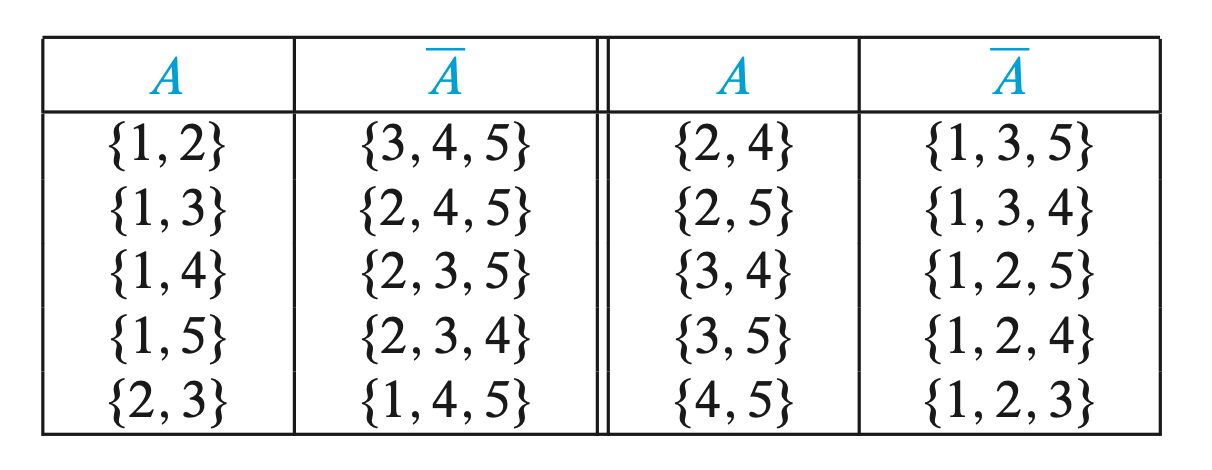
\includegraphics[width=.45\textwidth]{images/symmetry_example}
        \end{center}
\end{myredbox}
\vfill 
\begin{mygreenbox}[title=Scheinerman Prop 17.7]
Let $n,k \in \mathbb{N}$ with $0 \leq k \leq n$.  Then 
\[ \binom{n}{k} =\binom{n}{n-k} \]
\end{mygreenbox}


\end{frame}


\begin{frame}{Pascal's Triangle}
\footnotesize 
\begin{minipage}{.5\textwidth}

\only<1->{
\begin{center}
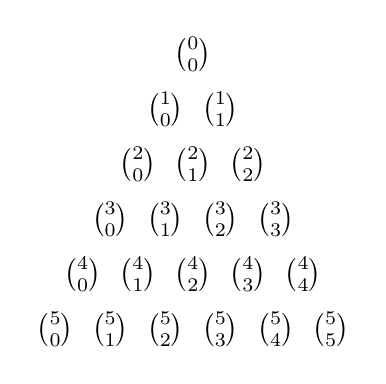
\begin{tikzpicture}[scale=0.7]
\foreach \n in {0,...,5} {
  \foreach \k in {0,...,\n} {
    \node at (\k-\n/2,-\n) {${\n \choose \k}$};
  }
}
\end{tikzpicture}
\end{center}
}
\end{minipage}
\hfill 
\begin{minipage}{.45\textwidth}
\only<2->{
\begin{center}
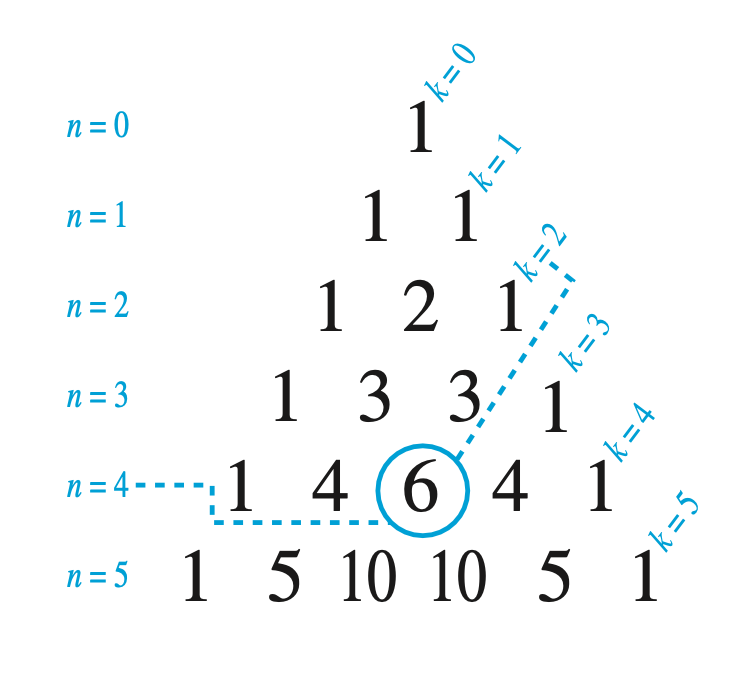
\includegraphics[width=.95\textwidth]{images/pascals_triangle.png}
\end{center}
}
\end{minipage}

\only<3->{\hfill \alert{Do you notice any pattern?} \hfill }

\only<4->{
\begin{myredbox}[title=Algorithm for forming Pascal's Triangle]
\begin{itemize}
\item Form an upside-down V shape of 1's.  (Why?)
\item The intermediate number in any row is formed by adding the two numbers just to its left and just to its right in the previous row.
\[ \binom{n}{k} =\binom{n-1}{k-1} + \binom{n-1}{k} \]
for integers $k$ and $n$ where $0 < k <n$.
\end{itemize}
\end{myredbox}
}



\end{frame}


\begin{frame}{Pascal's Triangle}
\footnotesize 
\begin{mygreenbox}[title=\text{Pascal's Identity}]
Let $k$ and $n$ be integers with $0 < k <n$. Then
\[ \binom{n}{k} =\binom{n-1}{k-1} + \binom{n-1}{k} \]
\end{mygreenbox}
\vfill 
\begin{myyellowbox}[title=\text{Poll: What is the intuition?}]
\pause 
Pick one of the elements to be \enquote{fire} (in the slang sense). 
\begin{itemize}
\item If we include the fire element in our selected subset, we have  $\binom{n-1}{k-1}$ ways to complete the subset.
\item If we don't include the fire element in our selected subset, then we have $ \binom{n-1}{k}$ ways to form the subset.
\end{itemize}

\end{myyellowbox}

\end{frame}


\begin{frame}{ Binomial Coefficients: Computational Formula}
\footnotesize 
\begin{mygreenbox}[title=\text{Scheinerman Thm 17.12: \quad Formula for $\binom{n}{k}$}]
Let $k$ and $n$ be integers with $0 \leq  k  \leq n$. Then
\[ \binom{n}{k} = \frac{n!}{k! (n-k)!} \]
\end{mygreenbox}
\vfill 
\begin{myyellowbox}[title=\text{Poll: How to understand this formula?}]
\pause 
\begin{enumerate} \footnotesize 
	\item Suppose we want to select $k$ items from a set of $n$ items, and \underline{order matters}.  Then the number of possible selections is
	%
	\begin{align*}
	(n)_k & = n \cdot (n-1) \cdot \hdots (n-k+1) && \scripttext{(From Sec. 8, Lists)} \\
	&= \frac{n!}{(n-k)!} && \scripttext{(Rewrite using factorial notation)}
	\end{align*}
	\item Now if \underline{order doesn't matter}, we \pause  need to treat all reorderings of the $k$ items as equivalent.  That is, we want to count equivalence classes, each of which has $k!$ members.  So by Scheinerman Theorem 16.6 (Counting equivalence classes), the total number of equivalence classes is $\frac{(n)_k}{k!}$.
\end{enumerate}
\footnotesize 
Hence, 
\[ \binom{n}{k} = \frac{(n)_k}{k!} = \frac{n!}{k! (n-k)!} \]
\end{myyellowbox}

\end{frame}

\begin{frame}{Application: Counting Lattice Paths}
\footnotesize 
\textbf{Problem.} Suppose we want to count the number of grid paths from the lower left corner to the upper right corner in which each step of the path either goes one unit to the right or one unit vertically. How many paths are there?
%
\begin{center}
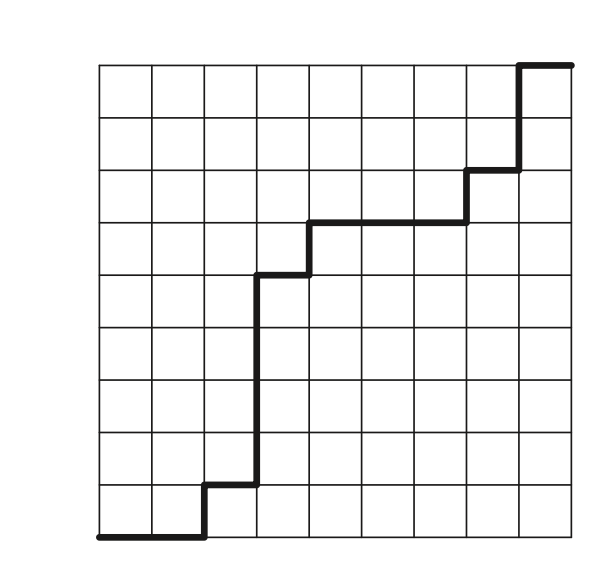
\includegraphics[width=.3\textwidth]{images/lattice_paths.png}
\end{center}
%
\vfill 
\pause 
\textbf{Solution.} Each possible path must take 18 steps - 9 rights and 9 ups.  Using \texttt{R} to denote right and \texttt{U} to denote up, one possible path is
\[\texttt{RRU RUU UUR URR RUR UUR} \]
Now we can count the number of paths by specifying which 9 of the 18 positions have \texttt{R}'s.  The solution is 
\pause 
\[ \binom{18}{9} = 48,620\]
\end{frame}


\begin{frame}[standout]
Group exercises
\end{frame}

\begin{frame}
\begin{columns}
\begin{column}{0.33\textwidth}
Ashley, Isabelle: 6 \\ 
Bailey, Tanna: 4 \\ 
Blaisdell, Olyver: 1 \\ 
Brown, Ashton: 12 \\ 
Brown, Jonathan: 6 \\ 
Cardenas, Dominic: 5 \\ 
Cutler, George: 5 \\ 
Fabik, Roland: 10 \\ 
Fellows, Audrey: 8 \\ 
Fitzgerald, Ryan: 11 \\ 
Fuller, Ryan: 4 \\ 
Griffen, Clara: 11 \\ 
Grutsch, Tanner: 9 \\\end{column}
\begin{column}{0.33\textwidth}
Hager, Nathan: 12 \\ 
Horner, Jayden: 7 \\ 
Johnson, Jaret: 10 \\ 
Kintzel, Samantha: 8 \\ 
Lameres, Alexis: 12 \\ 
Lee, Holden: 3 \\ 
Mayala, Reece: 3 \\ 
McLean, Connor: 4 \\ 
Mcbride, Daniel: 1 \\ 
Miller, Maverick: 2 \\ 
Moss, Emily: 8 \\ 
Mousseau, Matthew: 13 \\ 
Neuman, Evan: 9 \\\end{column}
\begin{column}{0.33\textwidth}
Putnam, John: 2 \\ 
Ramos, Vydel: 13 \\ 
Rathbun, Jedidiah: 13 \\ 
Roberts, Matthew: 11 \\ 
Roller, Nathan: 2 \\ 
Ryan, Otis: 9 \\ 
Shevtsov, Timothy: 1 \\ 
Sinclair, Aidan: 6 \\ 
Smith, Charles: 5 \\ 
Stensland, Emma: 7 \\ 
Thiessen, Logan: 10 \\ 
Thompson, Jaiden: 7 \\ 
Vath, Ethan: 3 \\\end{column}
\end{columns}
\end{frame}


\begin{frame}{Group exercises}
\footnotesize
\begin{enumerate}
	\item For each question below, determine the answer in three different ways.  First, write out all the possible subsets explicitly.  Second, use a proposition or theorem from the text.  Third, use a different proposition or theorem from the text.  

	\begin{itemize} \footnotesize 
	\item[a.] Determine the number of 2 element subsets of $\set{1,2,3,4,5,6}$.
	\item[b.] Determine the number of 4 element subsets of $\set{1,2,3,4,5,6}$.
	\end{itemize}
	\item Scheinerman Prop 17.7 says: Let $n,k \in \mathbb{N}$ with $0 \leq k \leq n$.  Then 
		\[ \binom{n}{k} = \binom{n}{n-k}. \]
	Prove this proposition using Scheinerman  Theorem 17.12, which says
		\[ \binom{n}{k} = \frac{n!}{k!(n-k)!}. \]
	\item Fifty runners compete in a 5K race.  How many different outcomes are possible? Find different answers according to the context. (a) We want to know in what place every runner finished.  (b) The race is a qualifying race, and we just want to pick the ten fastest runners. (c) The race is an Olympic final event, and we care only about who gets the gold, silver, and bronze medals.
	\item   At a large community festival, there’s a group of 30 volunteers — 8 from Missoula and 22 from other towns. The organizers want to form a five-person team to plan the main event. However, they insist that at least one person from Missoula must be on the team to make sure the town’s voice is heard. How many five-person teams can be formed containing at least one person from Missoula?
	\end{enumerate}

\end{frame}


\begin{frame}{Solution to group exercise \#1a}
\footnotesize

 There are 15 2-elements subsets of $\set{1,2,3,4,5,6}$.  We show this in 3 different ways. 
\begin{enumerate} 
	\item Writing out all the subsets explicitly, we have
%
\begin{align*}
\set{1,2}, \set{1,3}, \set{1,4}, \set{1,5}, \set{1,6} \\
\set{2,3}, \set{2,4}, \set{2,5}, \set{2,6} \\
\set{3,4}, \set{3,5}, \set{3,6} \\
\set{4,5}, \set{4,6} \\
\set{5,6} 
\end{align*}
%
\item The number of subsets of size 2 is given by Scheinerman Prop. 17.5 as 
\[ \binom{n}{2} = \sum_{k=1}^{n-1} k. \]
In this case, since $n=3$, we have $ \binom{6}{2} = 1+2+3=4+5 = 15.$
(Note that the layout of the solution to \#1 suggests why the formula is true.) 
\item The computational formula for $\binom{n}{k}$ (Scheinerman Theorem 17.12) is 
\[ \binom{n}{k}  = \frac{n!}{k! (n-k)!}\] 
Substituting $n=6$ and $k=2$, we find
%
\begin{align*}
\binom{6}{2} = \frac{6!}{2!4!} = \frac{6 \cdot 5}{2 \cdot 1} = 15. 
\end{align*}
\end{enumerate}
\end{frame}

\begin{frame}{Solution to group exercise \#1b}
\footnotesize

 There are 15 4-elements subsets of $\set{1,2,3,4,5,6}$.  We show this in 3 different ways. 
\begin{enumerate} 
	\item Writing out all the subsets explicitly, we have
%
\begin{align*}
\set{3,4,5,6}, \set{2,4,5,6}, \set{2,3,5,6}, \set{2,3,4,6}, \set{2,3,4,5} \\
\set{1,4,5,6}, \set{1,3,5,6}, \set{1,3,4,6}, \set{1,3,4,5} \\
\set{1,2,5,6}, \set{1,2,4,6}, \set{1,2,4,5} \\
\set{1,2,3,6}, \set{1,2,3,5} \\
\set{1,2,3,4} 
\end{align*}
%
\item Scheinerman Prop. 17.7  says that for $n,k \in \mathbb{N}$ with $0 \leq k \leq n$, we have  
\[ \binom{n}{k} = \binom{n}{n-k}\]
Hence  $\binom{6}{4} = \binom{6}{2}$. Since we already know from group exercise \#1a that $\binom{6}{2}=15$, we must have  $\binom{6}{4}=15$. (Indeed, the enumeration of subsets above was obtained by taking the complement of the enumerated subsets from the previous slide.) 
\item The computational formula for $\binom{n}{k}$ (Scheinerman Theorem 17.12) is 
\[ \binom{n}{k}  = \frac{n!}{k! (n-k)!}\] 
Substituting $n=6$ and $k=4$, we find
%
\begin{align*}
\binom{6}{2} = \frac{6!}{4!2!} = \frac{6 \cdot 5}{2 \cdot 1} = 15. 
\end{align*}
\end{enumerate}
\end{frame}

\begin{frame}{Solution to group exercise \#2}
\textbf{Problem.} Scheinerman Prop 17.7 says: Let $n,k \in \mathbb{N}$ with $0 \leq k \leq n$.  Then 
		\[ \binom{n}{k} = \binom{n}{n-k}. \]
	Prove this proposition using Scheinerman  Theorem 17.12. 
\vfill 
\textbf{Solution.} Scheinerman  Theorem 17.12 says
		\[ \binom{n}{k} = \frac{n!}{k!(n-k)!}. \] 
	If we apply Scheinerman  Theorem 17.12 to the problem of finding subsets of size $n-k$ from a set of size $n$, we have
	\[ \binom{n}{n-k} = \frac{n!}{(n-k)!\big(n-(n-k) \big)!} = \frac{n!}{(n-k)!k!} = \frac{n!}{k!(n-k)!}.  \]
Hence,
\[ \binom{n}{k} = \binom{n}{n-k}. \]
			
\end{frame}


\begin{frame}{Solution to group exercise \#3}
\textbf{Problem.}
Fifty runners compete in a 5K race.  How many different outcomes are possible? Find different answers according to the context. (a) We want to know in what place every runner finished.  (b) The race is a qualifying race, and we just want to pick the ten fastest runners. (c) The race is an Olympic final event, and we care only about who gets the gold, silver, and bronze medals.

\vfill 
\textbf{Solution.}
\begin{itemize}
\item[a.] $50!$. Here we want the number of permutations of the 50 runners; that is the number of different ways to order them. 
\item[b.]  Assuming that we don't care about the order in which the 10 runners finished, the answer is $\binom{50}{10}$. Here we want to find the number of subsets of size 10 from a pool of size 50.  (If we do care about the order in which the 10 runners finished, the answer is $50 \times 49 \times \cdots 41$.)
\item[c.] $50 \times 49 \times 48$. There are 50 choices for the first medal, which leaves 49 choices for the second medal and 48 choices for the third medal. 
\end{itemize}
\end{frame}


\begin{frame}{Solution to group exercise \#4}
\small 
\textbf{Problem.}
At a large community festival, there’s a group of 30 volunteers — 8 from Missoula and 22 from other towns. The organizers want to form a five-person team to plan the main event. However, they insist that at least one person from Missoula must be on the team to make sure the town’s voice is heard. How many five-person teams can be formed containing at least one person from Missoula?

\vfill 
\textbf{Solution.}  Let $T$ be the total number of five-person teams.  Let $M$ be the number of five-person teams with at least one person from Missoula.   Let $N$ be the number of five-person teams can with no people from Missoula.  Then
\[ M = T - N. \]

Now $T=\binom{30}{5}$ by definition of the binomial coefficient. (Here we can choose our five-person team from any of the 30 volunteers). Similarly,  $N=\binom{22}{5}$. (Here we must choose our five-person team solely from the 22 volunteers aren't from Missoula). Hence,
\[M = \binom{30}{5} - \binom{22}{5}. \] 


\end{frame}

\end{document}
